
%% bare_conf.tex
%% V1.3
%% 2007/01/11
%% by Michael Shell
%% See:
%% http://www.michaelshell.org/
%% for current contact information.
%%
%% This is a skeleton file demonstrating the use of IEEEtran.cls
%% (requires IEEEtran.cls version 1.7 or later) with an IEEE conference paper.
%%
%% Support sites:
%% http://www.michaelshell.org/tex/ieeetran/
%% http://www.ctan.org/tex-archive/macros/latex/contrib/IEEEtran/
%% and
%% http://www.ieee.org/

%%*************************************************************************
%% Legal Notice:
%% This code is offered as-is without any warranty either expressed or
%% implied; without even the implied warranty of MERCHANTABILITY or
%% FITNESS FOR A PARTICULAR PURPOSE!
%% User assumes all risk.
%% In no event shall IEEE or any contributor to this code be liable for
%% any damages or losses, including, but not limited to, incidental,
%% consequential, or any other damages, resulting from the use or misuse
%% of any information contained here.
%%
%% All comments are the opinions of their respective authors and are not
%% necessarily endorsed by the IEEE.
%%
%% This work is distributed under the LaTeX Project Public License (LPPL)
%% ( http://www.latex-project.org/ ) version 1.3, and may be freely used,
%% distributed and modified. A copy of the LPPL, version 1.3, is included
%% in the base LaTeX documentation of all distributions of LaTeX released
%% 2003/12/01 or later.
%% Retain all contribution notices and credits.
%% ** Modified files should be clearly indicated as such, including  **
%% ** renaming them and changing author support contact information. **
%%
%% File list of work: IEEEtran.cls, IEEEtran_HOWTO.pdf, bare_adv.tex,
%%                    bare_conf.tex, bare_jrnl.tex, bare_jrnl_compsoc.tex
%%*************************************************************************

% *** Authors should verify (and, if needed, correct) their LaTeX system  ***
% *** with the testflow diagnostic prior to trusting their LaTeX platform ***
% *** with production work. IEEE's font choices can trigger bugs that do  ***
% *** not appear when using other class files.                            ***
% The testflow support page is at:
% http://www.michaelshell.org/tex/testflow/



% Note that the a4paper option is mainly intended so that authors in
% countries using A4 can easily print to A4 and see how their papers will
% look in print - the typesetting of the document will not typically be
% affected with changes in paper size (but the bottom and side margins will).
% Use the testflow package mentioned above to verify correct handling of
% both paper sizes by the user's LaTeX system.
%
% Also note that the "draftcls" or "draftclsnofoot", not "draft", option
% should be used if it is desired that the figures are to be displayed in
% draft mode.
%
\documentclass[conference]{IEEEtran}
% Add the compsoc option for Computer Society conferences.
%
% If IEEEtran.cls has not been installed into the LaTeX system files,
% manually specify the path to it like:
% \documentclass[conference]{../sty/IEEEtran}





% Some very useful LaTeX packages include:
% (uncomment the ones you want to load)


% *** MISC UTILITY PACKAGES ***
%
%\usepackage{ifpdf}
% Heiko Oberdiek's ifpdf.sty is very useful if you need conditional
% compilation based on whether the output is pdf or dvi.
% usage:
% \ifpdf
%   % pdf code
% \else
%   % dvi code
% \fi
% The latest version of ifpdf.sty can be obtained from:
% http://www.ctan.org/tex-archive/macros/latex/contrib/oberdiek/
% Also, note that IEEEtran.cls V1.7 and later provides a builtin
% \ifCLASSINFOpdf conditional that works the same way.
% When switching from latex to pdflatex and vice-versa, the compiler may
% have to be run twice to clear warning/error messages.






% *** CITATION PACKAGES ***
%
%\usepackage{cite}
% cite.sty was written by Donald Arseneau
% V1.6 and later of IEEEtran pre-defines the format of the cite.sty package
% \cite{} output to follow that of IEEE. Loading the cite package will
% result in citation numbers being automatically sorted and properly
% "compressed/ranged". e.g., [1], [9], [2], [7], [5], [6] without using
% cite.sty will become [1], [2], [5]--[7], [9] using cite.sty. cite.sty's
% \cite will automatically add leading space, if needed. Use cite.sty's
% noadjust option (cite.sty V3.8 and later) if you want to turn this off.
% cite.sty is already installed on most LaTeX systems. Be sure and use
% version 4.0 (2003-05-27) and later if using hyperref.sty. cite.sty does
% not currently provide for hyperlinked citations.
% The latest version can be obtained at:
% http://www.ctan.org/tex-archive/macros/latex/contrib/cite/
% The documentation is contained in the cite.sty file itself.






% *** GRAPHICS RELATED PACKAGES ***
%
\ifCLASSINFOpdf
  % \usepackage[pdftex]{graphicx}
  % declare the path(s) where your graphic files are
  % \graphicspath{{../pdf/}{../jpeg/}}
  % and their extensions so you won't have to specify these with
  % every instance of \includegraphics
  % \DeclareGraphicsExtensions{.pdf,.jpeg,.png}
\else
  % or other class option (dvipsone, dvipdf, if not using dvips). graphicx
  % will default to the driver specified in the system graphics.cfg if no
  % driver is specified.
  % \usepackage[dvips]{graphicx}
  % declare the path(s) where your graphic files are
  % \graphicspath{{../eps/}}
  % and their extensions so you won't have to specify these with
  % every instance of \includegraphics
  % \DeclareGraphicsExtensions{.eps}
\fi
% graphicx was written by David Carlisle and Sebastian Rahtz. It is
% required if you want graphics, photos, etc. graphicx.sty is already
% installed on most LaTeX systems. The latest version and documentation can
% be obtained at:
% http://www.ctan.org/tex-archive/macros/latex/required/graphics/
% Another good source of documentation is "Using Imported Graphics in
% LaTeX2e" by Keith Reckdahl which can be found as epslatex.ps or
% epslatex.pdf at: http://www.ctan.org/tex-archive/info/
%
% latex, and pdflatex in dvi mode, support graphics in encapsulated
% postscript (.eps) format. pdflatex in pdf mode supports graphics
% in .pdf, .jpeg, .png and .mps (metapost) formats. Users should ensure
% that all non-photo figures use a vector format (.eps, .pdf, .mps) and
% not a bitmapped formats (.jpeg, .png). IEEE frowns on bitmapped formats
% which can result in "jaggedy"/blurry rendering of lines and letters as
% well as large increases in file sizes.
%
% You can find documentation about the pdfTeX application at:
% http://www.tug.org/applications/pdftex





% *** MATH PACKAGES ***
%
%\usepackage[cmex10]{amsmath}
% A popular package from the American Mathematical Society that provides
% many useful and powerful commands for dealing with mathematics. If using
% it, be sure to load this package with the cmex10 option to ensure that
% only type 1 fonts will utilized at all point sizes. Without this option,
% it is possible that some math symbols, particularly those within
% footnotes, will be rendered in bitmap form which will result in a
% document that can not be IEEE Xplore compliant!
%
% Also, note that the amsmath package sets \interdisplaylinepenalty to 10000
% thus preventing page breaks from occurring within multiline equations. Use:
%\interdisplaylinepenalty=2500
% after loading amsmath to restore such page breaks as IEEEtran.cls normally
% does. amsmath.sty is already installed on most LaTeX systems. The latest
% version and documentation can be obtained at:
% http://www.ctan.org/tex-archive/macros/latex/required/amslatex/math/





% *** SPECIALIZED LIST PACKAGES ***
%
%\usepackage{algorithmic}
% algorithmic.sty was written by Peter Williams and Rogerio Brito.
% This package provides an algorithmic environment fo describing algorithms.
% You can use the algorithmic environment in-text or within a figure
% environment to provide for a floating algorithm. Do NOT use the algorithm
% floating environment provided by algorithm.sty (by the same authors) or
% algorithm2e.sty (by Christophe Fiorio) as IEEE does not use dedicated
% algorithm float types and packages that provide these will not provide
% correct IEEE style captions. The latest version and documentation of
% algorithmic.sty can be obtained at:
% http://www.ctan.org/tex-archive/macros/latex/contrib/algorithms/
% There is also a support site at:
% http://algorithms.berlios.de/index.html
% Also of interest may be the (relatively newer and more customizable)
% algorithmicx.sty package by Szasz Janos:
% http://www.ctan.org/tex-archive/macros/latex/contrib/algorithmicx/




% *** ALIGNMENT PACKAGES ***
%
%\usepackage{array}
% Frank Mittelbach's and David Carlisle's array.sty patches and improves
% the standard LaTeX2e array and tabular environments to provide better
% appearance and additional user controls. As the default LaTeX2e table
% generation code is lacking to the point of almost being broken with
% respect to the quality of the end results, all users are strongly
% advised to use an enhanced (at the very least that provided by array.sty)
% set of table tools. array.sty is already installed on most systems. The
% latest version and documentation can be obtained at:
% http://www.ctan.org/tex-archive/macros/latex/required/tools/


%\usepackage{mdwmath}
%\usepackage{mdwtab}
% Also highly recommended is Mark Wooding's extremely powerful MDW tools,
% especially mdwmath.sty and mdwtab.sty which are used to format equations
% and tables, respectively. The MDWtools set is already installed on most
% LaTeX systems. The lastest version and documentation is available at:
% http://www.ctan.org/tex-archive/macros/latex/contrib/mdwtools/


% IEEEtran contains the IEEEeqnarray family of commands that can be used to
% generate multiline equations as well as matrices, tables, etc., of high
% quality.


%\usepackage{eqparbox}
% Also of notable interest is Scott Pakin's eqparbox package for creating
% (automatically sized) equal width boxes - aka "natural width parboxes".
% Available at:
% http://www.ctan.org/tex-archive/macros/latex/contrib/eqparbox/





% *** SUBFIGURE PACKAGES ***
%\usepackage[tight,footnotesize]{subfigure}
% subfigure.sty was written by Steven Douglas Cochran. This package makes it
% easy to put subfigures in your figures. e.g., "Figure 1a and 1b". For IEEE
% work, it is a good idea to load it with the tight package option to reduce
% the amount of white space around the subfigures. subfigure.sty is already
% installed on most LaTeX systems. The latest version and documentation can
% be obtained at:
% http://www.ctan.org/tex-archive/obsolete/macros/latex/contrib/subfigure/
% subfigure.sty has been superceeded by subfig.sty.



%\usepackage[caption=false]{caption}
%\usepackage[font=footnotesize]{subfig}
% subfig.sty, also written by Steven Douglas Cochran, is the modern
% replacement for subfigure.sty. However, subfig.sty requires and
% automatically loads Axel Sommerfeldt's caption.sty which will override
% IEEEtran.cls handling of captions and this will result in nonIEEE style
% figure/table captions. To prevent this problem, be sure and preload
% caption.sty with its "caption=false" package option. This is will preserve
% IEEEtran.cls handing of captions. Version 1.3 (2005/06/28) and later
% (recommended due to many improvements over 1.2) of subfig.sty supports
% the caption=false option directly:
%\usepackage[caption=false,font=footnotesize]{subfig}
%
% The latest version and documentation can be obtained at:
% http://www.ctan.org/tex-archive/macros/latex/contrib/subfig/
% The latest version and documentation of caption.sty can be obtained at:
% http://www.ctan.org/tex-archive/macros/latex/contrib/caption/




% *** FLOAT PACKAGES ***
%
%\usepackage{fixltx2e}
% fixltx2e, the successor to the earlier fix2col.sty, was written by
% Frank Mittelbach and David Carlisle. This package corrects a few problems
% in the LaTeX2e kernel, the most notable of which is that in current
% LaTeX2e releases, the ordering of single and double column floats is not
% guaranteed to be preserved. Thus, an unpatched LaTeX2e can allow a
% single column figure to be placed prior to an earlier double column
% figure. The latest version and documentation can be found at:
% http://www.ctan.org/tex-archive/macros/latex/base/



%\usepackage{stfloats}
% stfloats.sty was written by Sigitas Tolusis. This package gives LaTeX2e
% the ability to do double column floats at the bottom of the page as well
% as the top. (e.g., "\begin{figure*}[!b]" is not normally possible in
% LaTeX2e). It also provides a command:
%\fnbelowfloat
% to enable the placement of footnotes below bottom floats (the standard
% LaTeX2e kernel puts them above bottom floats). This is an invasive package
% which rewrites many portions of the LaTeX2e float routines. It may not work
% with other packages that modify the LaTeX2e float routines. The latest
% version and documentation can be obtained at:
% http://www.ctan.org/tex-archive/macros/latex/contrib/sttools/
% Documentation is contained in the stfloats.sty comments as well as in the
% presfull.pdf file. Do not use the stfloats baselinefloat ability as IEEE
% does not allow \baselineskip to stretch. Authors submitting work to the
% IEEE should note that IEEE rarely uses double column equations and
% that authors should try to avoid such use. Do not be tempted to use the
% cuted.sty or midfloat.sty packages (also by Sigitas Tolusis) as IEEE does
% not format its papers in such ways.





% *** PDF, URL AND HYPERLINK PACKAGES ***
%
%\usepackage{url}
% url.sty was written by Donald Arseneau. It provides better support for
% handling and breaking URLs. url.sty is already installed on most LaTeX
% systems. The latest version can be obtained at:
% http://www.ctan.org/tex-archive/macros/latex/contrib/misc/
% Read the url.sty source comments for usage information. Basically,
% \url{my_url_here}.





% *** Do not adjust lengths that control margins, column widths, etc. ***
% *** Do not use packages that alter fonts (such as pslatex).         ***
% There should be no need to do such things with IEEEtran.cls V1.6 and later.
% (Unless specifically asked to do so by the journal or conference you plan
% to submit to, of course. )


% correct bad hyphenation here
\hyphenation{op-tical net-works semi-conduc-tor}

\usepackage{algpseudocode}
\usepackage{algorithm}
\usepackage{subfig}
\usepackage{amsthm}
\usepackage{graphicx}
\usepackage{multirow}
\theoremstyle{definition}
\newtheorem{definition}{Definition}
\newtheorem*{theorem}{Theorem}


\begin{document}
%
% paper title
% can use linebreaks \\ within to get better formatting as desired
\title{Generating strategies for incremental covering array}


% author names and affiliations
% use a multiple column layout for up to three different
% affiliations
\author{\IEEEauthorblockN{Xintao Niu and Changhai nie}
\IEEEauthorblockA{State Key Laboratory for Novel \\
Software Technology\\
Nanjing University, China, 210023\\
Email: changhainie@nju.edu.com}
\and
\IEEEauthorblockN{Hareton Leung}
\IEEEauthorblockA{Department of computing \\
Hong Kong Polytechnic University\\
Kowloon, Hong Kong\\
Email: cshleung@comp.polyu.edu.hk
\and
\IEEEauthorblockN{Jeff Y. Lei}
\IEEEauthorblockA{Department of Computer Science\\
and Engineering\\
The University of Texas at Arlington\\
Email: ylei@cse.uta.edu}
}}
% conference papers do not typically use \thanks and this command
% is locked out in conference mode. If really needed, such as for
% the acknowledgment of grants, issue a \IEEEoverridecommandlockouts
% after \documentclass

% for over three affiliations, or if they all won't fit within the width
% of the page, use this alternative format:
%
%\author{\IEEEauthorblockN{Michael Shell\IEEEauthorrefmark{1},
%Homer Simpson\IEEEauthorrefmark{2},
%James Kirk\IEEEauthorrefmark{3},
%Montgomery Scott\IEEEauthorrefmark{3} and
%Eldon Tyrell\IEEEauthorrefmark{4}}
%\IEEEauthorblockA{\IEEEauthorrefmark{1}School of Electrical and Computer Engineering\\
%Georgia Institute of Technology,
%Atlanta, Georgia 30332--0250\\ Email: see http://www.michaelshell.org/contact.html}
%\IEEEauthorblockA{\IEEEauthorrefmark{2}Twentieth Century Fox, Springfield, USA\\
%Email: homer@thesimpsons.com}
%\IEEEauthorblockA{\IEEEauthorrefmark{3}Starfleet Academy, San Francisco, California 96678-2391\\
%Telephone: (800) 555--1212, Fax: (888) 555--1212}
%\IEEEauthorblockA{\IEEEauthorrefmark{4}Tyrell Inc., 123 Replicant Street, Los Angeles, California 90210--4321}}




% use for special paper notices
%\IEEEspecialpapernotice{(Invited Paper)}




% make the title area
\maketitle


\begin{abstract}
%\boldmath
Combinatorial testing (CT) is an effective technique for testing the interactions of factors in the software under test (SUT). By designing an efficient set of test cases, i.e., covering array, CT aims to check every possible validate interactions in SUT. Most existing covering array generating algorithms require a given \emph{degree} \emph{t} in prior, such that only the interactions with no more than $t$ factors are to be checked.  In practice, however, such $t$ cannot be properly determined, especially for systems with complicated interactions space.  Hence, incremental arrays are preferred. In this paper, we proposed two strategies for generating incremental covering arrays which can increase the coverage criteria when required. A preliminary evaluation of the two strategies is presented, which showed that, in consideration of the size of the covering array, both two strategies have their own advantages.
\end{abstract}
% IEEEtran.cls defaults to using nonbold math in the Abstract.
% This preserves the distinction between vectors and scalars. However,
% if the conference you are submitting to favors bold math in the abstract,
% then you can use LaTeX's standard command \boldmath at the very start
% of the abstract to achieve this. Many IEEE journals/conferences frown on
% math in the abstract anyway.

% no keywords




% For peer review papers, you can put extra information on the cover
% page as needed:
% \ifCLASSOPTIONpeerreview
% \begin{center} \bfseries EDICS Category: 3-BBND \end{center}
% \fi
%
% For peerreview papers, this IEEEtran command inserts a page break and
% creates the second title. It will be ignored for other modes.
\IEEEpeerreviewmaketitle



\section{Introduction}
With the growing complexity and scale of modern software systems, various factors, such as input values and configure options, can affect the behaviour of the system. Worse, some interactions between them can trigger unexpected negative effects on the software. To ensure the correctness and quality of the software system, it is desirable to detect and locate these \emph{bad} interactions. The simplest way to solve this problem is to perform exhaustive testing for all the possible validate interactions of the software system. It is, however, not impractical due to the combinatorial explosion. Therefore, to select a group of representative test cases from the whole testing space is required.

Combinatorial testing has been proven to be effective in identifying a good sample \cite{nie2011survey}. It works by generating a relatively small set of test cases, i.e., covering array, to test a group of particular interactions in the system. The number of factors involved in those selected interactions is limited in a moderate range, which is usually from 2 to 6 \cite{kuhn2002investigation}.

% The justification behind of this range is that based on empirical studies \cite{kuhn2002investigation}, most failures in the system are caused by the interactions with number of involved factors no more than 6 \cite{kuhn2002investigation}. And hence can fulfil testing requirement at most time.

Many algorithms are proposed to generate covering arrays. Apart from many differences between them,  those works have a common condition, i.e., they all need to be given a degree \emph{t} in prior.  The degree \emph{t} indicated the largest number of factors involved in the interactions to be covered, and the corresponding covering arrays which can satisfy this coverage criteria is called \emph{t}-way covering arrays. In practice, however, such a \emph{t} can not be properly determined. There are two reasons for this. First, many software systems suffer from complicated interactions space which make it challenging to estimate \emph{t}. In such case, even experienced testers can make mistakes and estimate a wrong value for \emph{t}, which can significantly affect the effectiveness and efficiency of CT. Specifically, if $t$ is estimated to be too large than required, many redundant test cases will be generated, which is a waste of computing resource. And if $t$ is estimated to be too small, then the generated covering array is not sufficient to obtain an effective testing targeting fault detection. Second, even though \emph{t} has been properly determined, there may not be enough time to completely execute all the test cases in the covering array. This is because testing software only makes sense before the next version is released. This time interval between two release versions may sometimes be too short for a complete testing of a high-way covering array \cite{fouche2009incremental}.

%In fact, in the worst case, any interaction with any strength can have an distinct affect of the SUT.

To make up for these shortcomings of traditional covering arrays, the incremental covering array \cite{fouche2009incremental} has been proposed. Such object can be deemed as adaptive covering array, which can increase the degree \emph{t} when required. As it can generate higher way covering array based on lower way covering array, it can reduce the cost when comparing with generating multiple ways of covering arrays. Additionally, it can be better applied on testing the software of which the released time is  frequently changed and cannot be predicted. Another advantage for generating incremental covering array is that testers can detect most faults in the software as soon as possible. This is because according to \cite{kuhn2002investigation}, most faults (about 70\% to 80\%) are caused by two-degree interactions, and almost all the faults can be covered by 6-way covering arrays. As incremental covering arrays first cover those lower-degree interactions, then the faults caused by them will be detected sooner.


In consideration of the size of the overall test cases, we argue that this approach of generating incremental covering array may produce too many test cases. This can be easily understood, as generating higher-way covering array based on the lower-way covering array (called \emph{bottom-up} strategy later) does not aim to optimize the size of the higher-way covering array. As a result, it may generate more test cases than those approaches that focus on generating a particular higher-way covering array.

Then a nature question, and also the motivation of this paper is, \textbf{is it possible to generate an incremental covering array with the same number of the overall test cases as those by the particular high-way covering array generating algorithms ?}  Before answering this question, one obvious conclusion to note is that any high way covering array must cover all the lower way interactions. So the answer for the previous question is \emph{yes}, as we just need apply a particular covering array generating algorithm to generate the high-way covering array, and then generate the lower-way covering arrays by extracting some subset of the test cases which can cover all the lower degree interactions. Later we call this strategy \emph{top-down}.

In this paper, we implemented these two strategies and evaluated their performance by comparing them at constructing several incremental covering arrays. The results of the experiments showed that the \emph{top-down} strategy has an significant advantage at the size of the higher-way covering array, while the \emph{bottom-up} strategy is better at constructing those lower-way covering arrays with smaller size.

%The answer is yes.
%For this, And also the key idea of this paper : To generate higher strength covering array from the lower strength, may be not effective at the size of the overall needed test cases. This can be easily understood, as it is not focus on the  higher covering array, which should . to in the .
%
%Then a . In fact, to execute the test cases , not mean to generate them in the order.


% no \IEEEPARstart
%Modern software are becoming more and more complicated. Combinatorial testing, as a black, has been proven to be effecive.
%
%
%and hence makes applying CT a challenge task.
%
%
%In the other hand, simply generated different covering arrays will be , as many test cases in the covering array may be redundant.
Our contributions include:

 \begin{enumerate}
 \item  We proposed two strategies for generating incremental covering arrays.
 \item  We conducted a series of experiments to compare and evaluate these two strategies.
 \item  We offer a recommendation for selecting which strategy when generating incremental covering array in practice.
\end{enumerate}
%\section{Motivation}
%

\section{Background}
This section gives some formal definitions related to CT. Assume that the behaviour of SUT is influenced by \emph{k} parameters, and each parameter $p_{i}$ has $a_{i}$ discrete values from the finite set $V_{i}$, i.e., $a_{i}$ = $|V_{i}|$ ($i$ = 1,2,..k). Then a \emph{test case} of the SUT is a group of values that are assigned to each parameter, which can be denoted as ($v_{1}, v_{2}, ..., v_{k}$). An $t$-degree interaction can be formally denoted as $(-, ..., v_{n_{1}}, -, ..., v_{n_{2}},-, ...,v_{n_{t}}, -, ...)$, where some t parameters have fixed values and other irrelevant parameters are represented as "-". In fact, a test case can be regarded as a $k$-degree interaction.


\subsection{Covering array}

\begin{definition}A $t$-way \emph{covering array} $MCA(N; t, k,$ $(a_{1}, a_{2}, ..., a_{k})$) is test set in the form of $N \times k$ table, where each row represents a \emph{test case} and each column represents a parameter.  For any \emph{t} columns, each possible \emph{t}-degree interaction of the $t$ parameters must appear at least once. When $ a_{1} = a_{2} = ... = a_{k} = v $, $t$-way covering array can be denoted as $CA(N; t, k, v)$.
\end{definition}


For example, Table \ref{ica_example} (a) shows a 2-way covering array $CA(5;2,4,2)$ for the SUT with 4 binary parameters. For any two columns, any 2-degree interaction is covered.  Covering array has proven to be effective in detecting the failures caused by interactions of parameters of the SUT. Many existing algorithms focus on constructing covering arrays such that the number of test cases, i.e., $N$, can be as small as possible.


\subsection{Incremental covering array}

\begin{definition}
An incremental covering array $ICA([N_{t_{1}},$ $N_{t_{1} + 1},...,N_{t_{2}}];[t_{1},t_{2}]$ $, k, v)$ is also a test set in the form of $N_{t_{2}} \times k$ table, where $t_{1} < t_{2}$ and  $N_{t_{1}}<N_{t_{1} + 1} <$ $,...,$ $< N_{t_{2}}$.  In this table, the first $N_{t_{i}}$ lines is a covering array $CA(N_{t_{i}}; t_{1} + i, k , v)$.
\end{definition}


Table \ref{ica_example} shows an example of incremental covering array, in which the two-way covering array $CA(5;2,4,2)$ is a subset of the three-way covering array $CA(9;3,4,2)$, which is also an incremental covering array $ICA([5,9];[2,3],4,2)$.

\begin{table}[htbp]
  \small
  \centering
  \caption{Experiment of Incremental covering array}
  \label{ica_example}

    \begin{tabular}{c}
 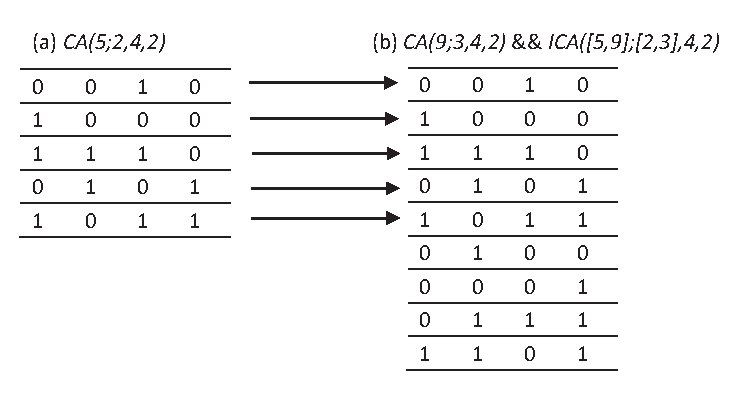
\includegraphics[width=3.4in]{incremental_covering_ex.eps}
    \end{tabular}%

\end{table}

%\begin{table}[htbp]
%  \small
%  \centering
%  \caption{Experiment of Incremental covering array}
%  \label{ica_example}
%  \subfloat[$CA(5;2,4,2)$]{%
%    \hspace{.5cm}%
%    \begin{tabular}{c c c c}
%        \hline
%
%        0 & 0 & 1 & 0 \\  \hline
%        1 & 0 & 0 & 0 \\ \hline
%        1 & 1 & 1 & 0 \\ \hline
%        0 & 1 & 0 & 1 \\ \hline
%        1 & 0 & 1 & 1 \\ \hline
%
%        \hline
%    \end{tabular}%
%    \hspace{.5cm}%
%  }\hspace{1cm}
%  \subfloat[$CA(9;3,4,2)$]{%
%    \hspace{.5cm}%
%    \begin{tabular}{c c c c}
%        \hline
%
%        0 & 0 & 1 & 0 \\  \hline
%        1 & 0 & 0 & 0 \\ \hline
%        1 & 1 & 1 & 0 \\ \hline
%        0 & 1 & 0 & 1 \\ \hline
%        1 & 0 & 1 & 1 \\ \hline
%        0 & 1 & 0 & 0 \\ \hline
%        0 & 0 & 0 & 1 \\ \hline
%        0 & 1 & 1 & 1 \\ \hline
%        1 & 1 & 0 & 1 \\ \hline
%
%    \end{tabular}%
%    \hspace{.5cm}%
%  }
%\end{table}


\begin{theorem}
Each $ICA([N_{t_{1}},N_{t_{1} + 1},...,N_{t_{2}}];[t_{1},t_{2}]$ $, k, v)$ is a $CA(N_{t_{2}}; t_{2}, k, v)$ covering array. Correspondingly, for each covering array $CA(N_{t_{2}}; t_{2}, k, v)$, we can find an $ICA([N_{t_{1}},N_{t_{1} + 1},...,N_{t_{2}}];[t_{1},t_{2}]$ $, k, v)$, s.t., the test cases of them are the same.
\end{theorem}

\begin{proof}
According to the definition of $ICA$, it can be easily got that $ICA([N_{t_{1}},N_{t_{1} + 1},...,N_{t_{2}}];[t_{1},t_{2}]$ $, k, v)$ is a $CA(N_{t_{2}}; t_{2}, k, v)$ covering array. For the second statement, we just need to prove that for any covering array, $CA(N_{t}; t, k, v)$, we can find a $CA(N_{t-1}; t-1, k, v)$, such that, $N_{t-1} < N_{t}$ and $\forall test\ case \in CA(N_{t-1}; t-1, k, v), test\ case\in CA(N_{t}; t, k, v)$.

 First, $CA(N_{t}; t, k, v)$  must be an $CA(N_{t}; t - 1, k, v)$, as it must cover all the $(t-1)$-degree interactions. Then assume to obtain a $(t-1)$-way covering array, any one test case in $CA(N_{t}; t - 1, k, v)$ can not be reduced. By this assumption, any test case will cover at least one $(t-1)$-degree interaction that only appears in this test case. Without loss of generality,  let test case  ($v_{1}, v_{2}, ..., v_{k}$) cover the $(t-1)$-degree interaction $(-, -, v_{3},.. -,...,v_{k})$ which only appears in the test case. Then obviously the $t$-degree interaction $(v_{1}', -, v_{3},.. -,...,v_{k})$  will never be covered by any test case in $CA(N_{t}; t, k, v)$, and hence $CA(N_{t}; t, k, v)$ is not a $t$-way covering array (Note this is based on that the parameter can take more than one value).

 It is contradiction, and means that we can reduce at least one test case in $CA(N_{t}; t - 1, k, v)$, so that it is still a $(t-1)$-way covering array.
\end{proof}

This theorem shows that the existence of the incremental covering arrays. As discussed before, generating the incremental covering arrays is of importance, as it supports adaptively increasing the coverage strength. By this, when testing a SUT, testers can firstly execute the lowest-way covering array in the incremental covering arrays, and then execute additional test cases from those higher-way covering arrays as required. The reuse of previous executed test cases will reduce for cost generating multiple different-ways covering arrays.

\section{Generating incremental covering arrays}
This section presents two strategies to generate the incremental covering arrays. The first strategy; \emph{bottom-up} strategy starts from generating the lowest-way covering array and then the higher-way ones. The second strategy;  \emph{top-down} strategy firstly generated the highest-way covering array, then the lower-way covering array.

\subsection{Bottom-up strategy}
This strategy is listed as Algorithm 1.
\begin{algorithm}
  \caption{Bottom-up strategy}
  \begin{algorithmic}[1]
     \Require
     $Param$ \Comment{parameter values for the SUT}

     $t_{1}$ \Comment{the lowest way}
     %$s_{fixed}$ \Comment{fixed part}

     $t_{2}$ \Comment{the highest way}

     \Ensure  $ICA$ \Comment{the incremental covering arrays}

    % \While{\textbf{not} $t_{uncovered}$ is not empty}
      \State $ICA \leftarrow Empty Set$
       \For {$t_{i} = t_{1};\ t_{i} \leq  t_{2};\ t_{i}\ INC$}
         \State $CA_{i} \leftarrow  Empty Set $
         \If {$t_{i} == t_{1}$}
                \State $CA_{i} \leftarrow CA\_Gen(Param, t_{i})$
         \Else
             \State $CA_{i} \leftarrow CA\_Gen\_Seeds(Param, t_{i}, CA_{i - 1})$
        \EndIf

        \State $ICA.append(CA_{i})$
      \EndFor

     \State \Return $ICA$
  \end{algorithmic}
\end{algorithm}
The inputs for this algorithm consists of the values for each parameter of the SUT --$Param$,  the lowest way $t_{1}$ of the covering array in the incremental covering array, and the highest way $t_{2}$ of the covering array . The output of this algorithm is an incremental covering array -- $ICA$.

This algorithm generates the covering array from lower-way to higher-way (line 2). If the current coverage strength $t_{i}$ is equal to $t_{1}$, it just utilize a covering array generating algorithm to generate the particular covering array (line 4 - 5). Otherwise, it will first take the previous generated covering array $CA_{i - 1}$ as seeds, and then utilize covering array generation algorithm to append additional test cases to satisfy higher coverage criteria (line 6 - 7).
%the example for . Consider we are testing a object, initially, we believe 1 way is enough, but when we give so, it find that is not , then we must increase the , to three way. In such a case, to take a Coverin array to regenerate 3-way covering array is follish, as it may introuduce many redunenta.t For example, many 3 way schemas in fact have been checked before.
%
%Then it is of course we need to generate the coverin array based on the previous covering array, such that we can utilze the previous tesing results. For this, a natural idea, is to set the as the seeds, like this.

Fig.\ref{increase-example} presents an example for constructing $ICA([6,13,24];[2,4], 5, 2)$ by this strategy. In this example, the covering array generating algorithm used is AETG \cite{cohen1997aetg}. The two-way covering array (test cases $c_{1}$ to $c_{6}$) is directly generated, and the three-way covering array (test cases $c_{1}$ to $ c_{13}$) is generated by adding additional test cases (test cases $c_{7}$ to $c_{13}$) based on the previous two-way covering array. The four-way covering array (test cases $c_{1}$ to $c_{24}$) is constructed on the previous three-way covering array. In total, to reach the 4-way covering array, there needs 24 test cases for this strategy.
\begin{figure}
\center
 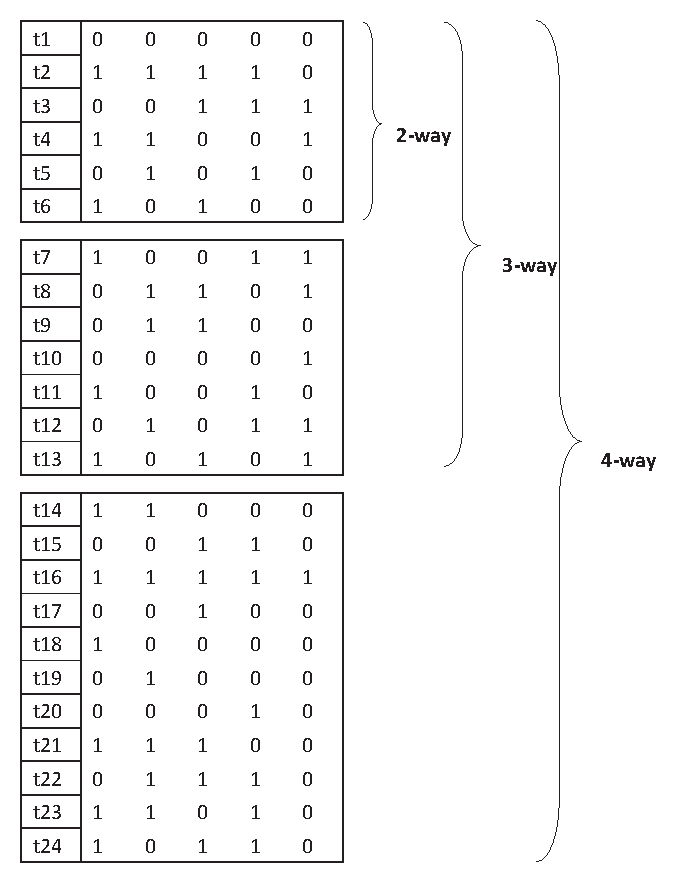
\includegraphics[width=3.0in]{increase_example.eps}
\caption{Bottom-up strategy example}
\label{increase-example}
\end{figure}

\subsection{Top-down strategy}
This strategy is listed as Algorithm 2, which generates covering arrays in the opposite order (line 2) against the previous strategy. Similarly, if the current coverage strength $t_{i}$ is equal to $t_{2}$, it directly generates the particular covering array (line 4 - 5). Otherwise, it will extract the covering array from a higher covering array ($CA_{i + 1}$) (line 6 - 10). The extraction process is a greedy approach. At each iteration, the test case which can cover most number of uncovered $t$-degree interactions will be selected from the higher-way covering array (line 7 - 10).  Note that this greedy selection does not promise to obtain the $CA_{i}$ covering array with the minimal size. But to get the minimal size, we need to exhaustive check every possible subset of the higher-covering array $CA_{i+1}$. This is impractical if the size of $CA_{i + 1}$ is too large.
%Another reason we does not focus on obtaining the minimal size of $CA_{i}$, is that even though we have, it does not have so that $CA_{i - 1}$.

%Now let us think the following problem, as the . If we had first generate the 3-way covering array, and .
%
%need to . And hence then , we need to increase the degree, as . To . Then first, a natural
\begin{algorithm}
  \caption{Top-down strategy}
  \begin{algorithmic}[1]
    \Require
     $Param$ \Comment{parameter values for the SUT}

     $t_{1}$ \Comment{the lowest way}
     %$s_{fixed}$ \Comment{fixed part}

     $t_{2}$ \Comment{the highest way}

     \Ensure  $ICA$ \Comment{the incremental covering arrays}

    % \While{\textbf{not} $t_{uncovered}$ is not empty}
      \State $ICA \leftarrow Empty Set$
       \For {$t_{i} = t_{2};\ t_{i} \geq  t_{1};\ t_{i}\  DEC $}
         \State $CA_{i} \leftarrow  Empty Set $
         \If {$t_{i} == t_{2}$}
                \State $CA_{i} \leftarrow CA\_Gen(Param, t_{i})$
         \Else
             \While{$t_{i}$-way coverage is not satisfied}
                \State $test \leftarrow selected\_best(CA_{i + 1})$
                \State $CA_{i}.append(test)$
             \EndWhile
        \EndIf

        \State $ICA.append(CA_{i})$
      \EndFor

     \State \Return $ICA$
  \end{algorithmic}
\end{algorithm}

An example for this strategy is given in Fig.\ref{decrease-example}. In this example, we first generated the highest-way covering array $CA(16; 4, 5, 2)$. Then we selected 14 test cases to form a three-covering array $CA(14; 3, 5, 2)$. Next the two-way covering array $CA(8; 2, 5, 2)$ is extracted from $CA(14; 3, 5, 2)$. The rows with dark background from the higher-way covering arrays represent those selected test cases.

\begin{figure}
 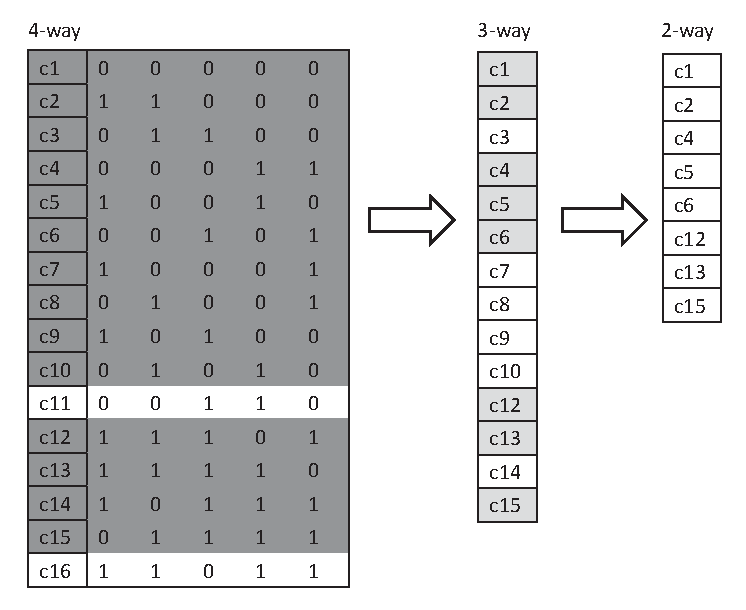
\includegraphics[width=3.4in]{decrease_example.eps}
\caption{Top-down strategy example}
\label{decrease-example}
\end{figure}


From the two examples, an obvious observation is that for the \emph{top-down} strategy, it has a significant advantage over the \emph{bottom-up} strategy with respect to the size of the highest-way covering array (16 for \emph{top-down} and 24 for \emph{bottom-up}). But when  considering the lower-way covering arrays, the \emph{bottom-up} performed better (13 and 6 for \emph{bottom-up}, while 14 and 8 for \emph{top-down} respectively).  To evaluate the generality of this observation , we conduct experiments in the next section.


%\section{}

\section{Preliminary Evaluation}
This section describes the experiments. We have prepared 9 SUT with their parameters as shown in Table \ref{ica_to_constuct}. The parameters are  presented in the abbreviated form $\#values^{\#number\ of\ parameters} ...$, e.g., $7^{3}6^{2}$ indicates the software has 3 parameters that can take 7 values and 2 parameters take 6 values. We didn't choose SUT with many parameter values because we will generate covering arrays with the coverage strength reaching to 5, which is quite time-consuming for AETG algorithm.

\begin{table}
\caption{The parameters of the SUT}
\label{ica_to_constuct}
\center
%\setlength{\tabcolsep}{3pt}
\begin{tabular}{c | c | c }
\hline  $SUT_{1}(4^{7}) $& $SUT_{2}(2^{15})$ & $SUT_{3}(2^{5}3^{2}5^{1})$ \\
\hline  $SUT_{4}(2^{10}3^{2})$ & $SUT_{5}(3^{7}4^{2})$ & $SUT_{6}(2^{8}9^{1})$ \\
\hline $SUT_{7}(2^{9}3^{2}5^{2})$ & $SUT_{8}(2^{8}4^{3})$ & $SUT_{9}(2^{8}3^{3}4^{1})$ \\
\hline
\end{tabular}
  \end{table}

Then for each SUT, we generate 4 incremental covering arrays, which are $ICA([N_{2},N_{3}]; [2, 3], k ,v)$, $ICA$ $([N_{2},$ $N_{3}$ $,N_{4}];[2, 3,4], k ,v)$, and $ICA([N_{2},N_{3},N_{4},N_{5}]$ $;[2,$ $ 3,4,5], k ,v)$, respectively. Each incremental covering array will be repeatedly generated 30 times by two strategies, and we will compare their average size. The results are shown in Table \ref{experiment_table}.

In this table, 


One observation is that the result is relatively stable. As the standard deviation is relatively small against the average amount of test cases.

With respect to the trend of average size, we post them in Fig\ref{experiement}.

 Fig.\ref{experiement}.

% Please add the following required packages to your document preamble:
% \usepackage{multirow}
\begin{table*}[h]
  \centering
  \caption{Experiment results}
  \label{experiment_table}
\begin{tabular}{|l|l|ll|lll|llll|}
\hline
\multicolumn{2}{|l|}{}            & \multicolumn{2}{l|}{$ICA([2, 3])$ (avg/stdev)}& \multicolumn{3}{l|}{$ICA$ $([2, 3,4])$ (avg/stdev)}    & \multicolumn{4}{l|}{$ICA([2, 3,4,5])$ (avg/stdev) }                   \\ \hline
\multirow{2}{*}{$SUT_{1}$} & Bottom-up & 26.2/0.91        & 126.07/2.16      & 26.73/1.12 & 127.13/2.38 & 519.23/3.88 & 26.8/0.95  & 125.9/1.62  & 519.9/0.95  & 1906.17/8.01  \\
                      & Top-down  & 30.87/1.06       & 123.53/2.46      & 30.77/0.8  & 137.93/1.95 & 509.23/0.8  & 30.17/1.04 & 139.13/1.93 & 553.07/1.04 & 1865.5/7.75   \\ \hline
\multirow{2}{*}{$SUT_{1}$} & Bottom-up & 85.53/1.98       & 226.23/3.95      & 85.87/2.03 & 227.1/4.78  & 703/7.51    & 86.1/1.76  & 227.8/4.28  & 704.07/1.76 & 1466.1/13.88  \\
                      & Top-down  & 90.03/0.75       & 167.87/3.3       & 84.93/1.88 & 244.47/2.26 & 661.93/1.88 & 84.1/1.58  & 246.63/2.39 & 610.27/1.58 & 1340.83/12.63 \\ \hline
\multirow{2}{*}{$SUT_{3}$} & Bottom-up & 17.27/0.96       & 54.13/1.71       & 17.03/0.98 & 54.97/1.97  & 138.37/3.02 & 16.97/0.87 & 55.13/1.89  & 138.93/0.87 & 302.23/5.04   \\
                      & Top-down  & 19.03/0.98       & 53.5/2.47        & 19.23/0.8  & 55.83/1.75  & 135.67/0.8  & 18.53/0.92 & 56.7/2.12   & 136.2/0.92  & 291.33/3.47   \\ \hline
\multirow{2}{*}{$SUT_{4}$} & Bottom-up & 12.23/1.05       & 32.97/1.2        & 12.8/1.22  & 33.27/1.44  & 87.1/4.37   & 12.67/1.11 & 33.13/1.65  & 87.5/1.11   & 212.13/7.91   \\
                      & Top-down  & 12.47/0.72       & 31.43/1.58       & 12.53/0.76 & 33.2/1.22   & 83.33/0.76  & 12.87/1.02 & 34.4/1.11   & 83.4/1.02   & 200.13/8.2    \\ \hline
\multirow{2}{*}{$SUT_{5}$} & Bottom-up & 21.9/1.47        & 85.4/2.12        & 21.67/1.11 & 85.73/1.93  & 307.9/3.46  & 21.73/1.34 & 85.63/2.17  & 306.7/1.34  & 984.1/6.39    \\
                      & Top-down  & 23.43/0.96       & 84.97/1.82       & 23.93/0.85 & 91.1/1.83   & 300.87/0.85 & 23.73/0.77 & 92.9/1.87   & 318.87/0.77 & 962.37/6.87   \\ \hline
\multirow{2}{*}{$SUT_{6}$} & Bottom-up & 85.9/1.72        & 228.27/3.63      & 86.5/2.01  & 226.97/3.7  & 701.57/7.93 & 86.1/1.49  & 226.23/3.78 & 700.6/1.49  & 1457.73/14.43 \\
                      & Top-down  & 90.17/0.58       & 167.13/2.2       & 85.5/2.14  & 244.33/2.05 & 663.53/2.14 & 83.8/1.7   & 245.87/2.95 & 612.07/1.7  & 1341.23/15.25 \\ \hline
\multirow{2}{*}{$SUT_{7}$} & Bottom-up & 29.53/2.12       & 100.33/2.57      & 29.33/2.33 & 100.67/2.71 & 336.8/7.07  & 29.27/2.06 & 100.43/3.19 & 334.53/2.06 & 953.97/15.52  \\
                      & Top-down  & 29/1.51          & 96.13/3.26       & 29.07/1.59 & 103/1.67    & 324.87/1.59 & 28.6/1.45  & 103.93/2.24 & 312.97/1.45 & 896.07/13.89  \\ \hline
\multirow{2}{*}{$SUT_{8}$} & Bottom-up & 21.13/1.12       & 76.83/4.45       & 21.2/0.95  & 75.23/3.4   & 218.27/4.84 & 21.17/1.29 & 75.7/3.56   & 216.23/1.29 & 557.53/9.34   \\
                      & Top-down  & 21.43/1.05       & 75.17/3.66       & 21.57/1.12 & 76.23/2.26  & 203.67/1.12 & 21.43/0.96 & 76.2/2.41   & 211.37/0.96 & 516.93/7.78   \\ \hline
\multirow{2}{*}{$SUT_{9}$} & Bottom-up & 17/0.89          & 55.03/1.72       & 17/0.89    & 55.13/1.02  & 167.1/4.22  & 16.6/0.71  & 54.6/1.76   & 164.83/0.71 & 444.1/9.64    \\
                      & Top-down  & 17.6/0.92        & 53.13/1.82       & 18.1/0.87  & 56.17/1.63  & 160.67/0.87 & 17.8/0.79  & 57.33/1.51  & 160.03/0.79 & 418.1/12.46   \\ \hline
\end{tabular}
\end{table*}

\begin{figure*}[htbp]
\center
 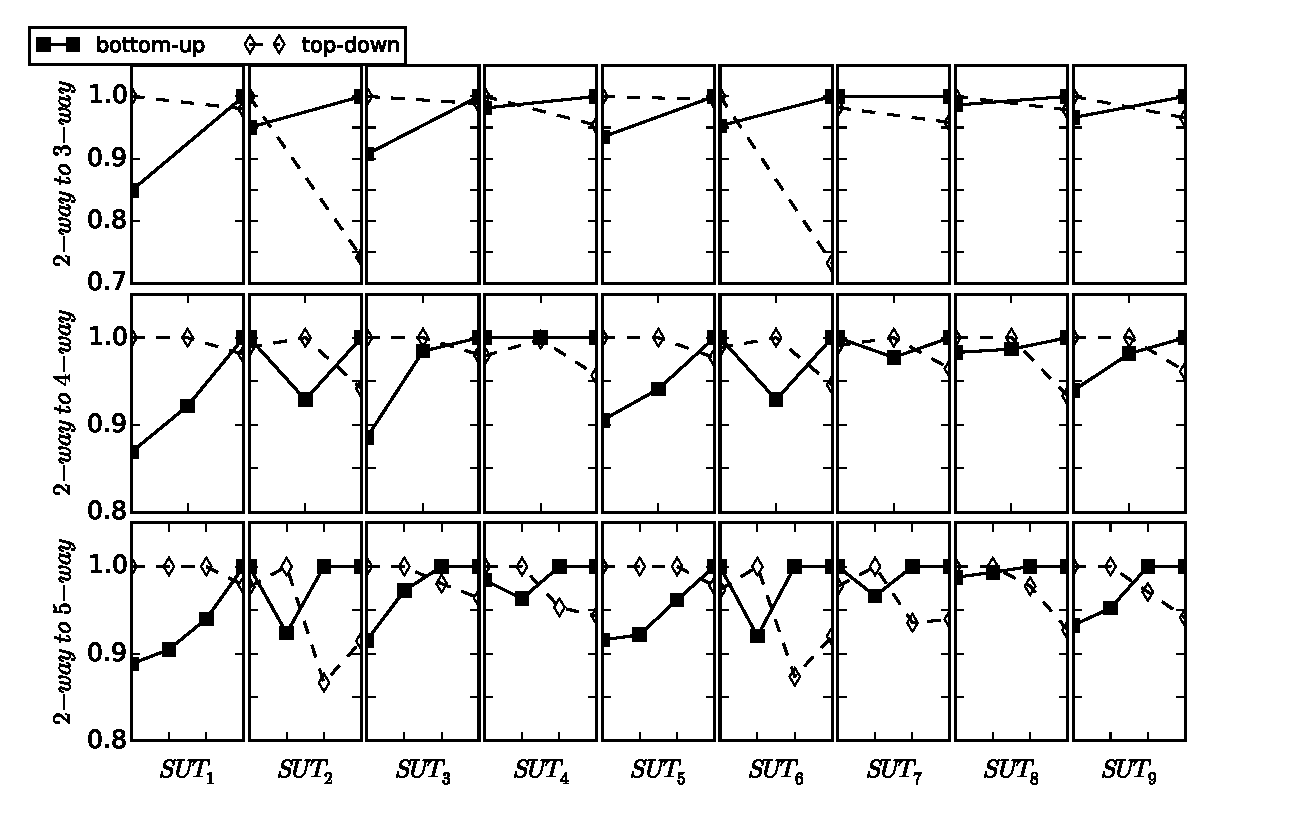
\includegraphics[width=6.0in]{experiment.eps}
\caption{Experiment results}
\label{experiement}
\end{figure*}


In Fig.\ref{experiement}, there are three main rows, representing the results of three incremental covering arrays , $ICA([N_{2},N_{3}]; [2, 3], k ,v)$, $ICA$ $([N_{2},$ $N_{3}$ $,N_{4}];[2, 3,4], k ,v)$, and $ICA([N_{2},N_{3},N_{4},N_{5}]$ $;[2,$ $ 3,4,5], k ,v)$, respectively.  The nine columns represents the nine SUTs in Table \ref{ica_to_constuct}. For each sub-figure in Fig.\ref{experiement}, the horizontal axis depicts the results of different-way covering array, and vertical axis represents size of the covering array. Note that we did not directly shows, instead, we normalize. This is because, the gap between the size of different-way covering array is too big to put into one figure.

From Fig.\ref{experiement}, we can observe that for most cases, \emph{top-down} strategy obtained smaller higher-way covering arrays (about 90 \% of that of \emph{bottom-up}), while \emph{bottom-up} strategy performed better at the lower-way covering arrays. This conclusion coincides with the case study presented in Section 3.  There are also some exceptions,; for example in the second row in Fig. \ref{experiement} ($ICA([N_{2},N_{3},N_{4}]; [2, 4], k ,v)$), \emph{top-down} strategy generated smaller 2-way covering arrays for $SUT_{2}$, $SUT_{4}$, and $SUT_{6}$ than that of \emph{bottom-up}. One possible explanation for the exception is that the covering array generated by greedy approach AETG sometimes may produce more test cases than needed.


Above all, the preliminary results suggested that when the coverage strength of the final covering array is low, \emph{bottom-up} strategy is preferred, otherwise, \emph{top-down} is a better choice.

%\begin{table}
%\caption{The incremental covering array to be constructed}
%\label{ica_to_constuct}
%\center
%\setlength{\tabcolsep}{3pt}
%\begin{tabular}{c | c | c }
%\hline  $ICA^{1}$:ICA((2,4),$10^{30}$)& $ICA^{2}$:ICA((2,4),$2^{100}$)& $ICA^{3}$:ICA((2,4),$10^{20}$) \\
%\hline  $ICA^{4}$:ICA((2,4),$7^{6}6^{7}5^{6}$) & $ICA^{5}$:ICA((2,4),$3^{13}$) & $ICA^{6}$:ICA((2,4),$8^{40}$ ) \\
%\hline  $ICA^{7}$:ICA((2,4),$15^{9}10^{6}$) & $ICA^{8}$:ICA((2,4),$4^{10}$) & $ICA^{9}$:ICA((2,4),$8^{20}$ ) \\
%\hline  $ICA^{10}$:ICA((2,4),$6^{10}$) & $ICA^{11}$:ICA((2,4),$4^{20}$) & $ICA^{12}$:ICA((2,4),$6^{20}$)\\\hline
%\end{tabular}
%  \end{table}

\section{Related work}
Nie et al. \cite{nie2011survey} gave a survey for combinatorial testing, in which the methods for generating covering
arrays are classified. Further Nie et al.\cite{nie2013adaptive} proposed a model for adaptive CT, in which the coverage strength of covering array needs to be adaptively changed as required.

S.Fouch{\'e}  et al. \cite{fouche2009incremental} proposed the incremental covering array, and gave a method to generate it. The method can be deemed as one special case of \emph{bottom-up} strategy, the only difference is that it used multiple lower-way covering arrays instead only one in this paper to construct the higher-way covering array. This is because their work needed to characterize the failure-inducing interactions in the covering array, in which ,multiple covering arrays can support a better diagnosis information.
%
%it hence use the classification tree method to classify the failure-inducing interaction, such that it should need to run multiple test cases, which is an augment of the bottom-up.


\section{Conclusions and future works}
This paper proposed two strategies for generating incremental covering arrays. Experimental results showed that both strategies have their own advantages; \emph{top-down} strategy is better at generating higher-way covering arrays, while \emph{bottom up} performed better at lower-way ones .

As a future work, we will apply more covering array generating algorithms, to compare their performance at generating incremental covering arrays. Another interesting work is to combine the two strategies, so that we can first select a median coverage strength \emph{t} and generate incremental covering arrays by \emph{top-down} strategy. Then if the maximal-way covering array is generated, we can use \emph{bottom-up} strategy to generate further higher-way covering arrays. We believe such a combination strategies may offer a better performance.
% An example of a floating figure using the graphicx package.
% Note that \label must occur AFTER (or within) \caption.
% For figures, \caption should occur after the \includegraphics.
% Note that IEEEtran v1.7 and later has special internal code that
% is designed to preserve the operation of \label within \caption
% even when the captionsoff option is in effect. However, because
% of issues like this, it may be the safest practice to put all your
% \label just after \caption rather than within \caption{}.
%
% Reminder: the "draftcls" or "draftclsnofoot", not "draft", class
% option should be used if it is desired that the figures are to be
% displayed while in draft mode.
%
%\begin{figure}[!t]
%\centering
%\includegraphics[width=2.5in]{myfigure}
% where an .eps filename suffix will be assumed under latex,
% and a .pdf suffix will be assumed for pdflatex; or what has been declared
% via \DeclareGraphicsExtensions.
%\caption{Simulation Results}
%\label{fig_sim}
%\end{figure}

% Note that IEEE typically puts floats only at the top, even when this
% results in a large percentage of a column being occupied by floats.


% An example of a double column floating figure using two subfigures.
% (The subfig.sty package must be loaded for this to work.)
% The subfigure \label commands are set within each subfloat command, the
% \label for the overall figure must come after \caption.
% \hfil must be used as a separator to get equal spacing.
% The subfigure.sty package works much the same way, except \subfigure is
% used instead of \subfloat.
%
%\begin{figure*}[!t]
%\centerline{\subfloat[Case I]\includegraphics[width=2.5in]{subfigcase1}%
%\label{fig_first_case}}
%\hfil
%\subfloat[Case II]{\includegraphics[width=2.5in]{subfigcase2}%
%\label{fig_second_case}}}
%\caption{Simulation results}
%\label{fig_sim}
%\end{figure*}
%
% Note that often IEEE papers with subfigures do not employ subfigure
% captions (using the optional argument to \subfloat), but instead will
% reference/describe all of them (a), (b), etc., within the main caption.


% An example of a floating table. Note that, for IEEE style tables, the
% \caption command should come BEFORE the table. Table text will default to
% \footnotesize as IEEE normally uses this smaller font for tables.
% The \label must come after \caption as always.
%
%\begin{table}[!t]
%% increase table row spacing, adjust to taste
%\renewcommand{\arraystretch}{1.3}
% if using array.sty, it might be a good idea to tweak the value of
% \extrarowheight as needed to properly center the text within the cells
%\caption{An Example of a Table}
%\label{table_example}
%\centering
%% Some packages, such as MDW tools, offer better commands for making tables
%% than the plain LaTeX2e tabular which is used here.
%\begin{tabular}{|c||c|}
%\hline
%One & Two\\
%\hline
%Three & Four\\
%\hline
%\end{tabular}
%\end{table}


% Note that IEEE does not put floats in the very first column - or typically
% anywhere on the first page for that matter. Also, in-text middle ("here")
% positioning is not used. Most IEEE journals/conferences use top floats
% exclusively. Note that, LaTeX2e, unlike IEEE journals/conferences, places
% footnotes above bottom floats. This can be corrected via the \fnbelowfloat
% command of the stfloats package.



% conference papers do not normally have an appendix


% use section* for acknowledgement
\section*{Acknowledgment}
This work was supported by the National Natural Science Foundation of China (No. 61272079), the Research Fund for the Doctoral Program of Higher Education of China (No.20130091110032), the Science Fund for Creative Research Groups of the National Natural Science Foundation of China(No. 61321491), and the Major Program of National Natural Science Foundation of China (No. 91318301)




% trigger a \newpage just before the given reference
% number - used to balance the columns on the last page
% adjust value as needed - may need to be readjusted if
% the document is modified later
%\IEEEtriggeratref{8}
% The "triggered" command can be changed if desired:
%\IEEEtriggercmd{\enlargethispage{-5in}}

% references section

% can use a bibliography generated by BibTeX as a .bbl file
% BibTeX documentation can be easily obtained at:
% http://www.ctan.org/tex-archive/biblio/bibtex/contrib/doc/
% The IEEEtran BibTeX style support page is at:
% http://www.michaelshell.org/tex/ieeetran/bibtex/
\bibliographystyle{IEEEtran}
% argument is your BibTeX string definitions and bibliography database(s)
\bibliography{incremental}
%
% <OR> manually copy in the resultant .bbl file
% set second argument of \begin to the number of references
% (used to reserve space for the reference number labels box)
%\begin{thebibliography}{1}
%
%\bibitem{IEEEhowto:kopka}
%H.~Kopka and P.~W. Daly, \emph{A Guide to \LaTeX}, 3rd~ed.\hskip 1em plus
%  0.5em minus 0.4em\relax Harlow, England: Addison-Wesley, 1999.
%
%\end{thebibliography}




% that's all folks
\end{document}


